
\quad 1.\quad Перейходим по ссылке https://www.virtualbox.org. Нажимаем кнопку “Download”, выбираем «Windows hosts» и устанавливаем «VirtualBox». 

\begin{figure}[h]	
		\centering
		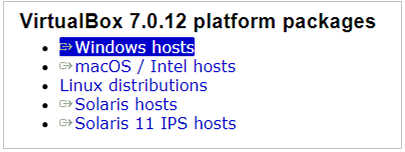
\includegraphics[width=0.5\linewidth]{VM/1.png}
\caption{«Windows hosts».}
\label{ris:image}
\end{figure}

\quad 2.\quad Далее, для того чтобы любая виртуальная машина могла работать, необходимо включить виртуализацию. Чтобы проверить, включена ли она, открываем диспетчер задач и переходим в раздел «Производительность». Открываем окно диспетчера задач на весь экран и внизу увидими, включена ли виртуализация.

\begin{figure}[h]
		\centering
		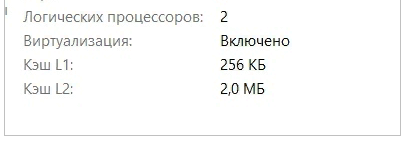
\includegraphics[width=0.5\linewidth]{VM/2.png}
\caption{Диспетчер задач. Виртуализация.}
\label{ris:image}
\end{figure}

\quad Если виртуализация выключена, то необходимо войти в BIOS. Для этого нужно нажать на кнопку «Перезагрузить компьютер», и, как только он начинает запускаться, зажать клавишу «Esc» ( или начать нажимать много раз на клавишу delete, пока не запустится «Startup menu». Зависит от того, ноутбук у вас или компьютер), после чего и откроется «Startup menu». Чтобы открыть BIOS нажмите клавишу «F10». Переходим в «System Configuration» нажав два раза на кнопку со стрелочкой вправо. Затем спускаемся до «Virtualization Technology», нажав на кнопку со стрелочкой вниз и нажимаем клавишу «Enter». Выбираем «Enable» и снова нажимаем «Enter». Нажимаем клавишу «F10» и выбираем «Yes». После чего компьютер перезагрузится уже с включённой виртуализацией.

\begin{figure}[h]
		\centering
		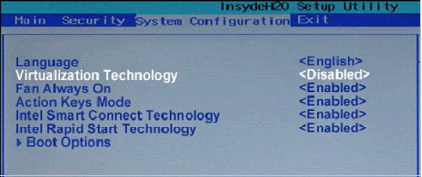
\includegraphics[width=0.5\linewidth]{VM/3.png}
\caption{BIOS. «Virtualization Technology».}
\label{ris:image}
\end{figure}

3. Скачиваем «Ubuntu» с официального сайта по ссылке: https://ubuntu.com/download/desktop. Затем открываем «VirtualBox» и нажимаем кнопку «Создать». Заполняя все поля, необходимо указать объём памяти не менее 2 гигабайт, иначе «Ubuntu» просто не запустится. В остальном можно принять все установки по умолчанию. После создания, необходимо нажать на кнопку «Настройки», далее «Носители», у надписи «Контроллер: IDE» нажать на значок диска с плюсиком. 

\begin{figure}[h]
		\centering
		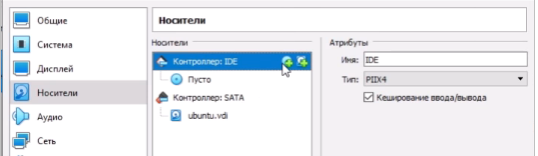
\includegraphics[width=0.65\linewidth]{VM/4.png}
\caption{Настройки. Носители.}
\label{ris:image}

\end{figure}

\quad Затем «Добавить» и выбрать скаченный ранее файл с «Ubuntu». После чего можно нажать кнопку «Запустить». После запуска, мы выбираем язык, нажимаем скачать «Ubuntu», заполняем все поля, и выбираем параметры по умолчанию. И наконец видим интерфейс «Linux».
